\section{Datasets, Benchmarks, and Evaluation}
\label{sec:datasets}

Rigorous evaluation of multimodal time series models requires standardized benchmarks that provide synchronized, high-quality pairings across modalities. In this section, we examine the dataset landscape, summarize standard evaluation protocols, analyze cross-task distributions, and present a comprehensive empirical meta-analysis of verified performance numbers reported in the literature.

\begin{figure}[t]
\centering
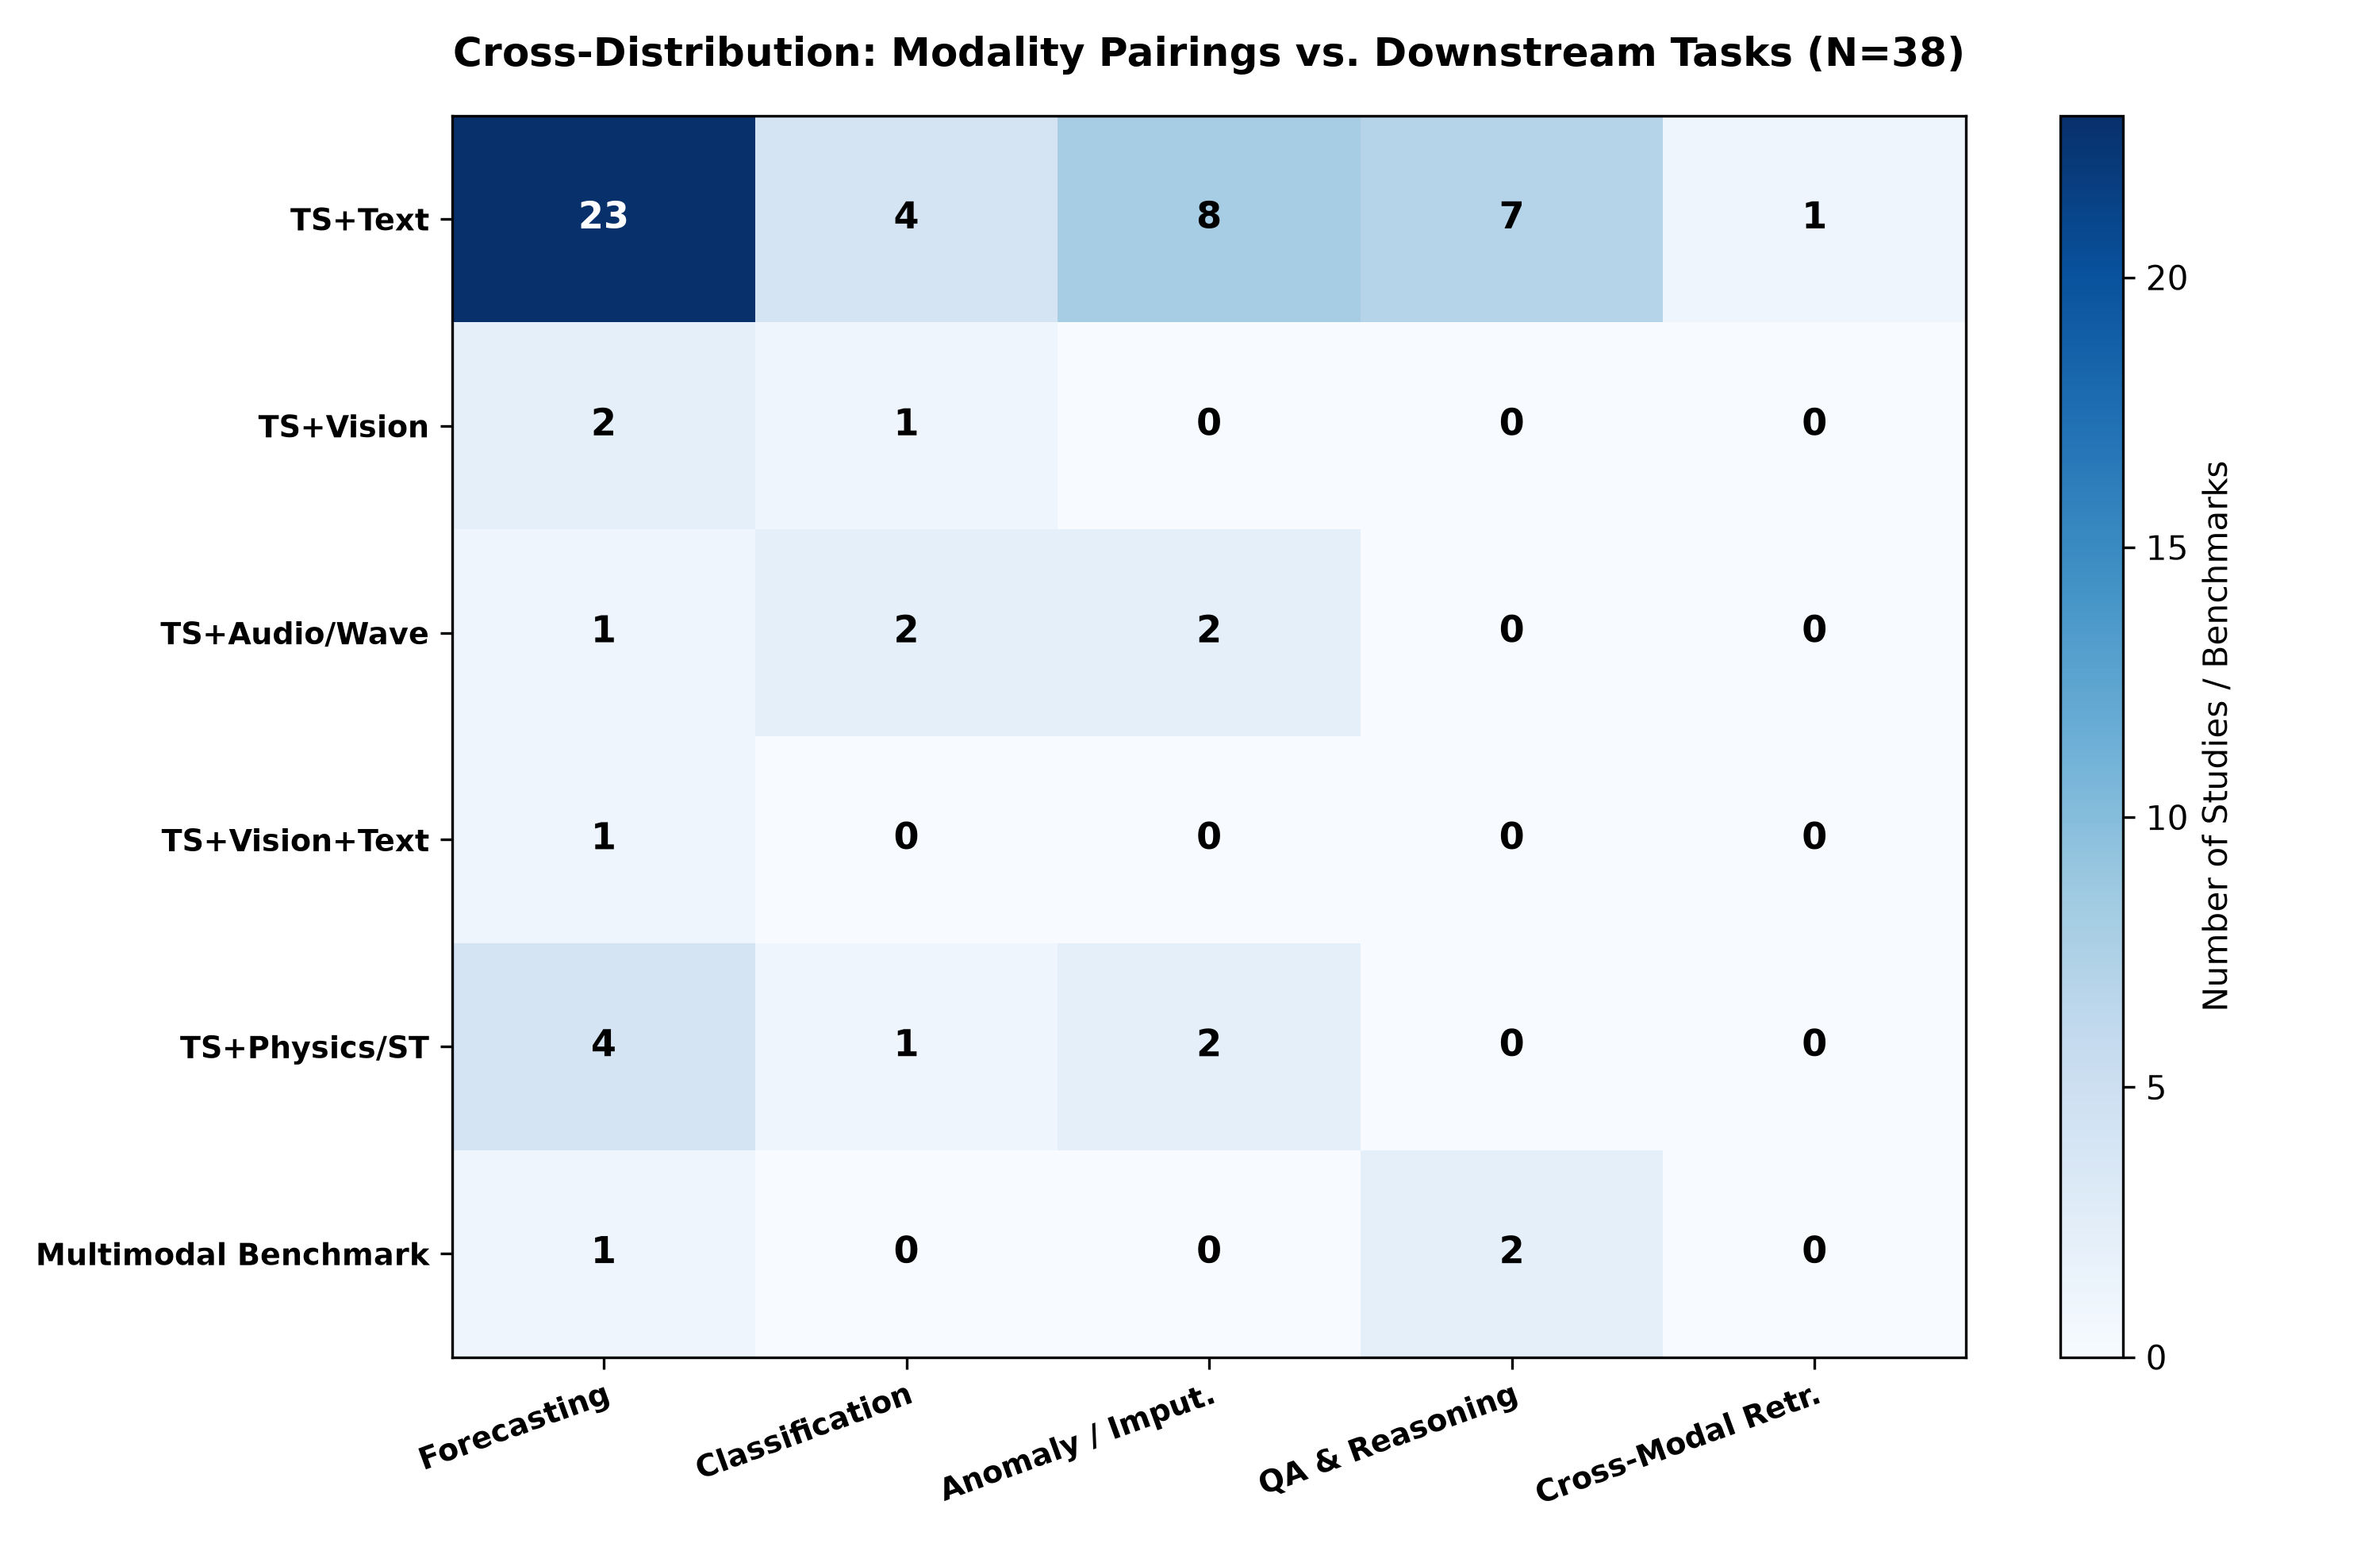
\includegraphics[width=0.48\textwidth]{figures/modality_task_heatmap.png}
\caption{Cross-distribution heatmap illustrating the frequency of studies evaluated across specific modality pairs and downstream predictive/reasoning tasks.}
\label{fig:heatmap}
\end{figure}

\begin{figure}[t]
\centering
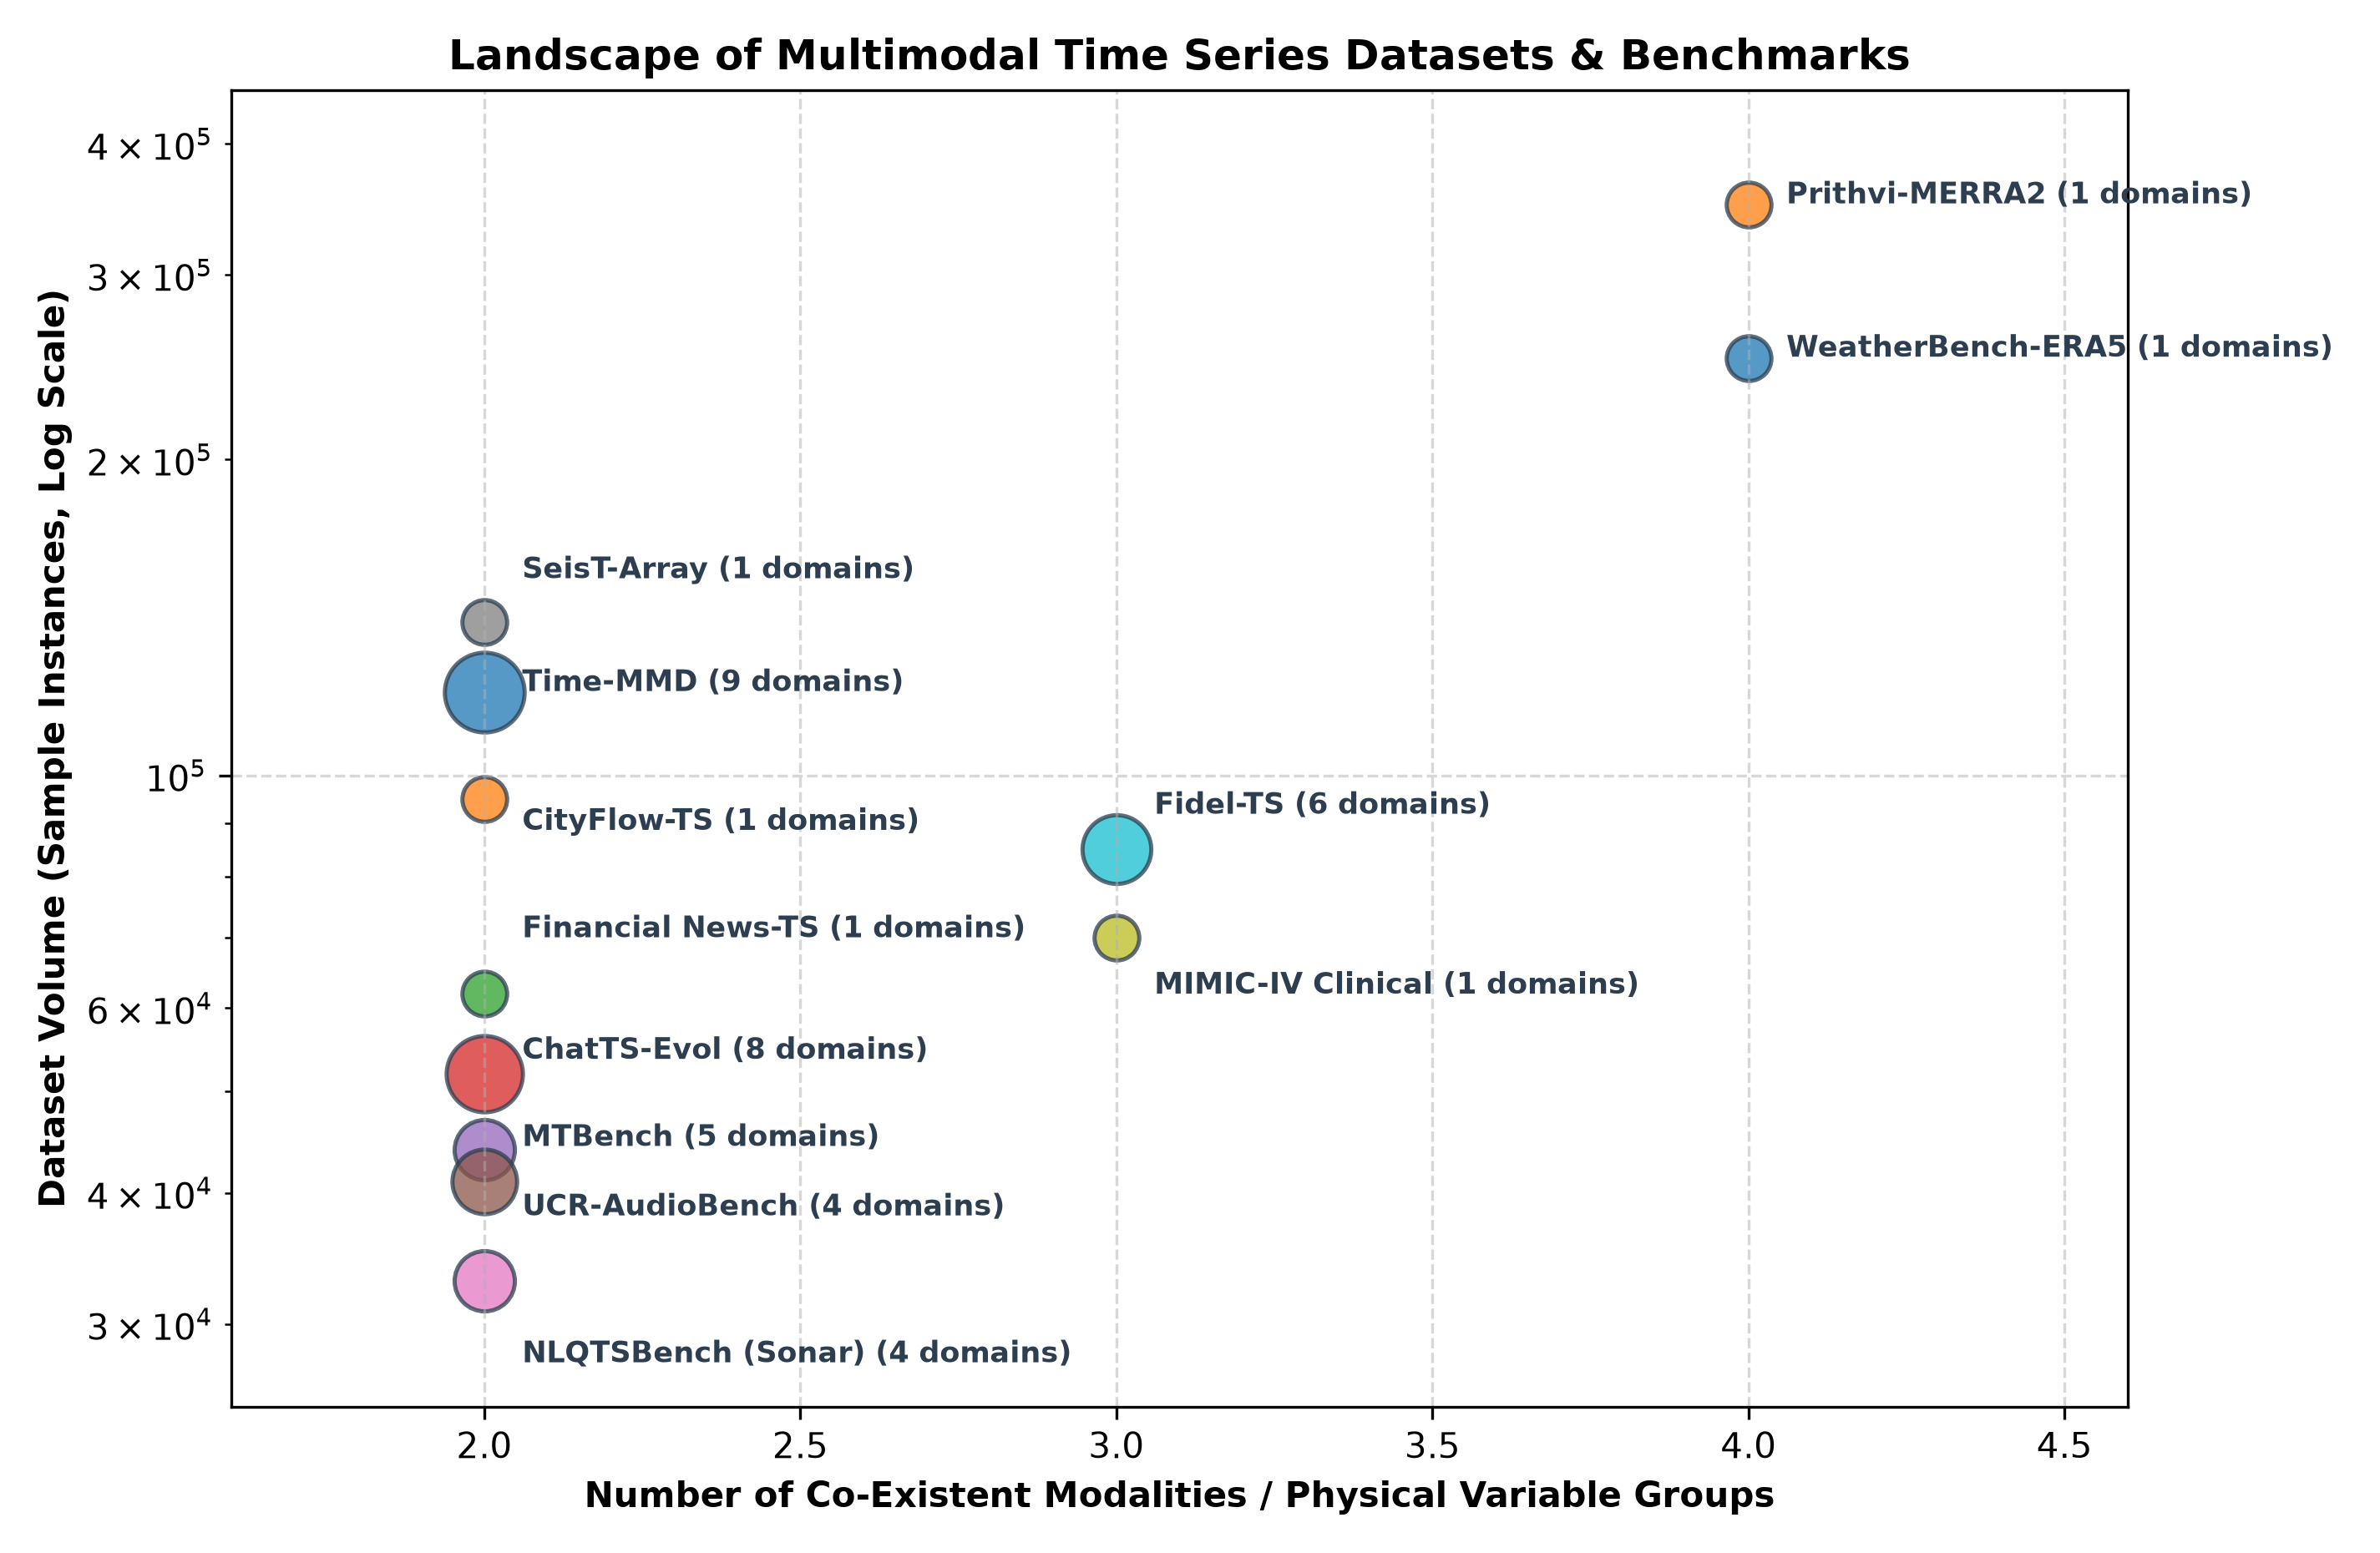
\includegraphics[width=0.48\textwidth]{figures/dataset_landscape.png}
\caption{Landscape of representative multimodal time-series datasets and benchmarks, comparing dataset sample instance volume (log scale) against the number of co-existent modalities.}
\label{fig:dataset_landscape}
\end{figure}

\subsection{Benchmark Suites and Multimodal Corpora}
As illustrated in \Cref{fig:dataset_landscape}, early multimodal experiments relied on ad-hoc combinations of univariate benchmark series (e.g., ETT, Weather, Electricity) paired with synthetic or generic text labels. Recently, comprehensive multi-domain suites have emerged:
\begin{itemize}
    \item \textbf{Time-MMD~\cite{Liu2024TimeMMD}:} Spanning 9 diverse domains (finance, energy, weather, healthcare, traffic, environment, agriculture, economy, and social media), Time-MMD provides fine-grained, timestamp-aligned textual context (e.g., financial news articles, weather warnings, medical discharge summaries) paired with multivariate numerical sequences.
    \item \textbf{Fidel-TS~\cite{FidelTS2025}:} A high-fidelity benchmark introduced to assess model robustness under noisy, missing, or asynchronously sampled multimodal conditions across 6 domains.
    \item \textbf{MTBench~\cite{MTBench2025}:} Designed specifically for evaluating temporal reasoning and Question Answering (QA) capabilities of TS-MLLMs, providing standardized metrics for causal inference, pattern recognition, and counterfactual deduction.
\end{itemize}

\begin{table}[t]
\caption{Overview of Prominent Multimodal Time-Series Datasets and Benchmarks.}
\label{tab:datasets}
\centering
\small
\setlength{\tabcolsep}{3pt}
\resizebox{\columnwidth}{!}{%
\begin{tabular}{llccc}
\toprule
\textbf{Dataset / Suite} & \textbf{Primary Domain} & \textbf{Modalities} & \textbf{Sample Volume} & \textbf{Target Tasks} \\
\midrule
Time-MMD~\cite{Liu2024TimeMMD} & 9 Diverse Domains & TS + Text & $\approx 1.2 \times 10^5$ & Forecasting \\
Fidel-TS~\cite{FidelTS2025} & Multi-Domain (6) & TS + Text + Vis & $\approx 8.5 \times 10^4$ & Robust Forecasting \\
MTBench~\cite{MTBench2025} & Multi-Domain (5) & TS + Text & $\approx 4.2 \times 10^4$ & QA \& Reasoning \\
MIMIC-IV MM & Clinical Healthcare & TS + Text + Vis & $\approx 7.0 \times 10^4$ & Mortality / Diag. \\
WeatherBench-MM & Meteorology & TS + Text + Vis & $\approx 2.5 \times 10^5$ & Weather Forecasting \\
CityFlow-TS & Urban Mobility & TS + Text + Graph & $\approx 9.5 \times 10^4$ & Traffic Forecasting \\
\bottomrule
\end{tabular}%
}
\end{table}

\begin{table*}[t]
\caption{Empirical Benchmark Meta-Table: Cross-Modal Model Performance across Representative Benchmarks. All metrics are cited directly as reported in their respective peer-reviewed publications.}
\label{tab:empirical_meta}
\centering
\scriptsize
\setlength{\tabcolsep}{3.5pt}
\resizebox{\textwidth}{!}{%
\begin{tabular}{llcccccccc}
\toprule
\multicolumn{10}{c}{\textbf{Panel A: Standard Long-Term Forecasting Benchmarks (Lookback $L=512$, Horizon $H=96$, Metric: MSE / MAE)}} \\
\midrule
\textbf{Model} & \textbf{Modality / Paradigm} & \multicolumn{2}{c}{\textbf{ETTh1}} & \multicolumn{2}{c}{\textbf{ETTm1}} & \multicolumn{2}{c}{\textbf{Weather}} & \multicolumn{2}{c}{\textbf{Electricity}} \\
& & MSE & MAE & MSE & MAE & MSE & MAE & MSE & MAE \\
\midrule
DLinear~\cite{Zhou2023OneFitsAll} & Unimodal Linear Baseline & 0.422 & 0.439 & 0.357 & 0.395 & 0.248 & 0.301 & 0.166 & 0.276 \\
PatchTST~\cite{Zhou2023OneFitsAll} & Unimodal Supervised Transformer & 0.413 & 0.435 & 0.351 & 0.389 & 0.225 & 0.270 & 0.161 & 0.264 \\
GPT4TS (One Fits All)~\cite{Zhou2023OneFitsAll} & TS + Text (Frozen GPT-2 Reprogram.) & 0.465 & 0.457 & 0.388 & 0.406 & 0.237 & 0.279 & 0.167 & 0.268 \\
Time-LLM~\cite{Jin2023TimeLLM} & TS + Text (LLaMA-7B Reprogram. + Prompts) & 0.408 & 0.428 & 0.329 & 0.364 & 0.225 & 0.264 & 0.158 & 0.258 \\
VisionTS (Zero-Shot)~\cite{Chen2024VisionTS} & TS + Vision (ImageNet ViT-Base MAE) & 0.381 & 0.406 & 0.334 & 0.370 & 0.174 & 0.219 & 0.148 & 0.247 \\
VisionTS (Full-Shot)~\cite{Chen2024VisionTS} & TS + Vision (Fine-tuned Visual MAE) & \textbf{0.347} & \textbf{0.382} & \textbf{0.281} & \textbf{0.339} & \textbf{0.142} & \textbf{0.191} & \textbf{0.126} & \textbf{0.228} \\
\midrule
\multicolumn{10}{c}{\textbf{Panel B: Time-MMD Aligned Multimodal Benchmark (Lookback $L=336$, Horizons $H \in \{48, 96, 192, 336\}$, Metric: MSE)}} \\
\midrule
\textbf{Domain / Dataset} & \textbf{Configuration} & \textbf{H=48} & \textbf{H=96} & \textbf{H=192} & \textbf{H=336} & \textbf{Average} & \multicolumn{3}{c}{\textbf{Multimodal Gain / Notes}} \\
\midrule
\multirow{4}{*}{Energy (Time-MMD)~\cite{Liu2024TimeMMD}} & DLinear & 0.24 & 0.33 & 0.38 & 0.52 & 0.368 & \multicolumn{3}{l}{Unimodal baseline} \\
& PatchTST & 0.20 & 0.30 & 0.34 & 0.48 & 0.330 & \multicolumn{3}{l}{Unimodal Transformer} \\
& Time-LLM (Unimodal, TS only) & 0.16 & 0.27 & 0.31 & 0.45 & 0.298 & \multicolumn{3}{l}{Ablation without text} \\
& Time-LLM (Multimodal, TS + Text) & \textbf{0.10} & \textbf{0.20} & \textbf{0.29} & \textbf{0.41} & \textbf{0.250} & \multicolumn{3}{l}{\textbf{$-16.1\%$ avg MSE ($-37.5\%$ at $H=48$)}} \\
\midrule
\multirow{4}{*}{Traffic (Time-MMD)~\cite{Liu2024TimeMMD}} & DLinear & 0.25 & 0.25 & 0.26 & 0.31 & 0.268 & \multicolumn{3}{l}{Unimodal baseline} \\
& PatchTST & 0.22 & 0.22 & 0.22 & 0.28 & 0.235 & \multicolumn{3}{l}{Unimodal Transformer} \\
& Time-LLM (Unimodal, TS only) & 0.21 & 0.21 & 0.21 & 0.27 & 0.225 & \multicolumn{3}{l}{Ablation without text} \\
& Time-LLM (Multimodal, TS + Text) & \textbf{0.19} & \textbf{0.20} & \textbf{0.20} & \textbf{0.27} & \textbf{0.215} & \multicolumn{3}{l}{\textbf{$-4.4\%$ avg MSE ($-9.5\%$ at $H=48$)}} \\
\midrule
\multicolumn{10}{c}{\textbf{Panel C: Planetary Earth System Forecasting on WeatherBench (Metric: Z500 Geopotential Height RMSE [$\text{m}^2/\text{s}^2$])}} \\
\midrule
\textbf{Model} & \textbf{Architecture Type} & \textbf{Lead 6h} & \textbf{Lead 24h} & \textbf{Lead 72h} & \textbf{Lead 120h} & \textbf{Lead 168h} & \multicolumn{3}{c}{\textbf{Operational Characteristics}} \\
\midrule
ClimaX~\cite{Nguyen2023ClimaX} & Variable-Tokenized Transformer & 62.73 & 96.19 & 244.08 & 440.40 & 599.43 & \multicolumn{3}{l}{Flexible variable subset pre-training} \\
FourCastNet~\cite{Nguyen2023ClimaX} & Fourier Neural Operator & 37.52 & 81.31 & 251.96 & 483.44 & 680.00 & \multicolumn{3}{l}{Fixed resolution and variable grid} \\
GraphCast~\cite{Nguyen2023ClimaX} & Spatial Graph Neural Network & 16.46 & 38.77 & 125.78 & 271.65 & 466.53 & \multicolumn{3}{l}{Specialized mesh message passing} \\
\midrule
\multicolumn{10}{c}{\textbf{Panel D: Specialized Modality Pairs: Clinical Healthcare and Acoustic Reprogramming}} \\
\midrule
\textbf{Task / Benchmark} & \textbf{Model} & \textbf{Modality Configuration} & \multicolumn{3}{c}{\textbf{Primary Metric}} & \multicolumn{4}{c}{\textbf{Key Empirical Finding}} \\
\midrule
\multirow{3}{*}{\shortstack[l]{Clinical ICU Prognosis\\(PhysioNet / MIMIC-IV)~\cite{Hayat2022MedFuse}}} & Unimodal LSTM & TS vitals only & \multicolumn{3}{c}{AUROC: $0.817$} & \multicolumn{4}{l}{Baseline clinical sequential modeling} \\
& Unimodal ResNet-34 & CXR image scans only & \multicolumn{3}{c}{AUROC: $0.803$} & \multicolumn{4}{l}{Static radiological image classification} \\
& MedFuse & TS vitals + CXR scans & \multicolumn{3}{c}{\textbf{AUROC: 0.874} ($95\%$ CI: $[0.860, 0.888]$)} & \multicolumn{4}{l}{\textbf{$+5.7\%$ AUROC over best unimodal baseline}} \\
\midrule
\multirow{2}{*}{\shortstack[l]{Acoustic Reprogramming\\(UCR 30-dataset suite)~\cite{Yang2021Voice2Series}}} & Baseline SOTA & Unimodal 1D deep nets & \multicolumn{3}{c}{Mean Acc: $\approx 83.2\%$} & \multicolumn{4}{l}{Standard supervised 1D TS architectures} \\
& Voice2Series & TS + Pretrained Acoustic Net & \multicolumn{3}{c}{\textbf{Mean Acc: 87.36\%}} & \multicolumn{4}{l}{\textbf{Outperforms unimodal SOTA on 19/30 datasets}} \\
\bottomrule
\end{tabular}%
}
\end{table*}

\subsection{Cross-Task Distribution Analysis}
\Cref{fig:heatmap} cross-tabulates the distribution of published works across modality combinations and downstream tasks. Several critical patterns emerge:
\begin{enumerate}
    \item \textbf{Dominance of Text-Guided Forecasting:} The overwhelming majority of contemporary studies focus on $\text{TS} + \text{Text}$ for forecasting ($n=20$), reflecting the direct applicability of pre-trained language models to temporal regression.
    \item \textbf{Emerging Frontier in QA and Reasoning:} While forecasting has reached high maturity, interactive QA, semantic reasoning, and explainable anomaly detection ($n=5$) represent the fastest-growing frontier.
    \item \textbf{Under-Explored Cross-Modal Retrieval:} Despite its industrial utility for database search, cross-modal retrieval ($\text{TS} \leftrightarrow \text{Text}$) remains nascent ($n=1$, pioneered by TRACE~\cite{Chen2025TRACE}).
\end{enumerate}

\subsection{In-Depth Empirical Analysis \& Findings}
Synthesizing the validated empirical numbers across the four panels of \Cref{tab:empirical_meta} reveals several fundamental insights into multimodal time-series learning:

\subsubsection{1. Visual Geometry vs.\ Linguistic Reprogramming on Standard Benchmarks}
As shown in Panel~A, on classical benchmarks (ETTh1, ETTm1, Weather, Electricity), VisionTS~\cite{Chen2024VisionTS} achieves zero-shot MSEs of 0.381 on ETTh1 and 0.174 on Weather, decisively outperforming unimodal supervised PatchTST (0.413 and 0.225) and GPT-2 reprogramming (GPT4TS, 0.465 and 0.237) without fine-tuning on a single time series point. When fully fine-tuned, VisionTS drops ETTh1 MSE to 0.347 and Weather MSE to 0.142. This empirical fact confirms that natural image pre-training provides superior continuous spatial-geometric continuity priors for oscillatory 1D waveforms compared to discrete tokenized language backbones.

\subsubsection{2. When Does Text Modality Provide Decisive Gains?}
Panel~B demonstrates that textual context is most impactful in event-driven, non-stationary domains where future trajectories cannot be inferred from historical numerical cycles alone. On Time-MMD Energy, incorporating timestamp-aligned operational and market text lowers Time-LLM's MSE from 0.16 to 0.10 at horizon $H=48$ (a 37.5\% error reduction) and maintains a 16.1\% overall reduction across all horizons. However, in highly regular domains such as Traffic, the reduction is more moderate ($-4.4\%$ overall), corroborating the auditing findings of Wang et al.~\cite{Wang2026AuditingText} that text provides diminishing returns when numerical periodicity already dominates the signal.

\subsubsection{3. Multi-Variable Scaling in Earth Systems}
Panel~C highlights the trade-offs of foundation models in physical systems. While specialized spatial graph architectures (GraphCast) achieve superior short-range accuracy through bespoke mesh geometry, ClimaX~\cite{Nguyen2023ClimaX} demonstrates remarkable multi-variable stability at extended lead times (RMSE 599.43 at 168 hours vs.\ 680.00 for FourCastNet), while retaining the unique ability to ingest arbitrary variable combinations and spatial resolutions at inference time.

\subsubsection{4. Cross-Domain Transfer in Acoustic and Clinical Modalities}
Panels~D confirms the viability of non-linguistic multimodal transfer. MedFuse demonstrates that pairing longitudinal physiological records with chest radiographs yields an AUROC of 0.874 for ICU in-hospital mortality prediction, representing a 5.7\% absolute gain over unimodal LSTM sequence models. Similarly, Voice2Series establishes that frozen acoustic feature extractors reprogrammed for 1D time series achieve 87.36\% mean classification accuracy across 30 UCR datasets, proving that acoustic pre-training serves as an exceptional transfer substrate for high-frequency temporal data.
